\documentclass{beamer}

\usepackage{hyperref}
\usepackage{url}

\newenvironment{itemframe}[1]{\begin{frame}{#1}\begin{itemize}}   {\end{itemize}\end{frame}}

\title{Sep 2 Prep Work}
\author{Michael Cardiff}
% \logo{\large \LaTeX{}}
\subtitle{PHYS 163a}

% Changes style of actual slides
\usetheme{Dresden}
% Changes color of slides
\usecolortheme{spruce}
% removes controls at bottom right side
\usenavigationsymbolstemplate{}

% for figures
\graphicspath{ {./figs/} }

\begin{document}

\begin{frame}
  \titlepage
\end{frame}

\section{What is Carnot's Engine?}
\begin{frame}{Kardar's Definition}
  \begin{center}
    \textit{A Carnot Engine is any engine that is \underline{reversible}, runs in a \underline{cycle}, with all of its \underline{heat exchanges} taking place at temperature $T_H$ and a sink temperature $T_C$}
  \end{center}
  We should break this down a bit
\end{frame}

\begin{frame}{Reversiblity}
  \begin{columns}
    \begin{column}{0.5\textwidth}
      \begin{itemize}
      \item Reversing a process = Going backward in time
      \item A reversible process can be run backward in time by swapping input and output
      \item For Carnot's engine, this means swapping $T_C$ with $T_H$ and vice versa
      \item Reversibility implies an Equilibrium
      \end{itemize}
    \end{column}
    \begin{column}{0.5\textwidth}
      \begin{figure}[H]
        \centering
        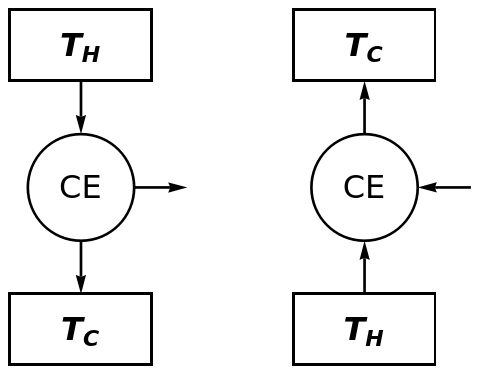
\includegraphics[width=5.0cm]{carnot.png}
        \caption{Carnot Engine and its reversal}
      \end{figure}
    \end{column}
  \end{columns}
  
\end{frame}

\begin{frame}{The Carnot Cycle}
    \begin{columns}
    \begin{column}{0.5\textwidth}
      \begin{itemize}
      \item Heat must be exchanged between two isotherms, at temperatures $T_H$ and $T_C$
      \item The Isotherms are then connected by \textit{adiabats} in which no heat is exchanged, this allows the cycle to close
      \item In The figure, the red lines are isoterms, and the blue are adiabats
      \end{itemize}
    \end{column}
    \begin{column}{0.5\textwidth}
      \begin{figure}[H]
        \centering
        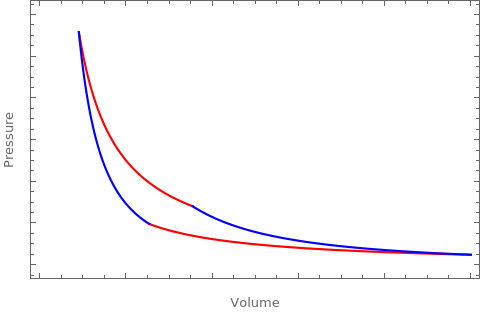
\includegraphics[width=5.0cm]{carnotcycle.png}
        \caption{Carnot Cycle Example}
      \end{figure}
    \end{column}
  \end{columns}  
\end{frame}

\begin{frame}{Heat Exchanging}
  \begin{itemize}
  \item While there is not net change during the adiabatic processes, there is during the isothermal processes
  \item Work is given off\footnote{In an engine} in order to actually cool the medium from $T_H$ to $T_C$
  \item Work is absorbed\footnote{In a refrigerator} into the system in order to cool $T_H$ down to $T_C$
  \end{itemize}
\end{frame}

\end{document}